実験1では, 認証機構が正しく機能していることを確認するための実験を
行った. 適度に影響が出るよう, 3章で述べた2種類の不正ノードを3個ずつ用意し, 
全ノードの約8\% (6個のノード)を不正ノードに設定した. また, 結果のばらつきを
抑えつつ, 統計的に有意な評価を可能にするために, そのような環境で
250回シミュレーションを行い, パケット配送率 (PDR)とスループットを
調べた. \\
\indent 実験の結果は以下の通りである. \\

\newpage
\begin{figure}
  \centering
  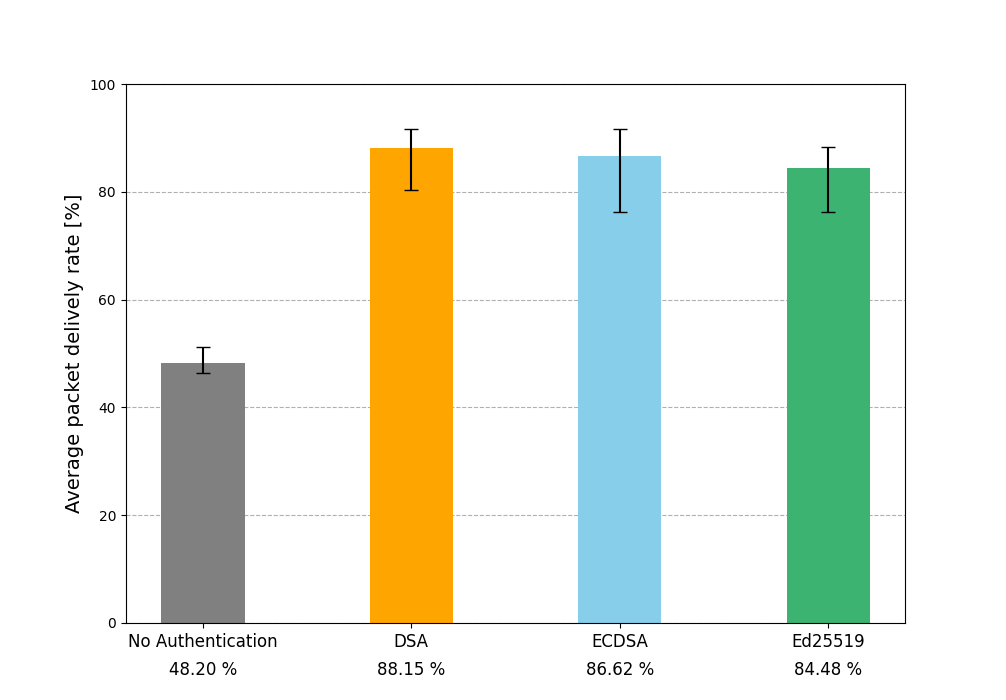
\includegraphics[width=1\textwidth]{figures/exp1_pdr.png}
  \caption{不正ノードが存在する環境でのパケット配送率}
  \label{fig:exp1_pdr}
\end{figure}
\clearpage
\begin{figure}
  \centering
  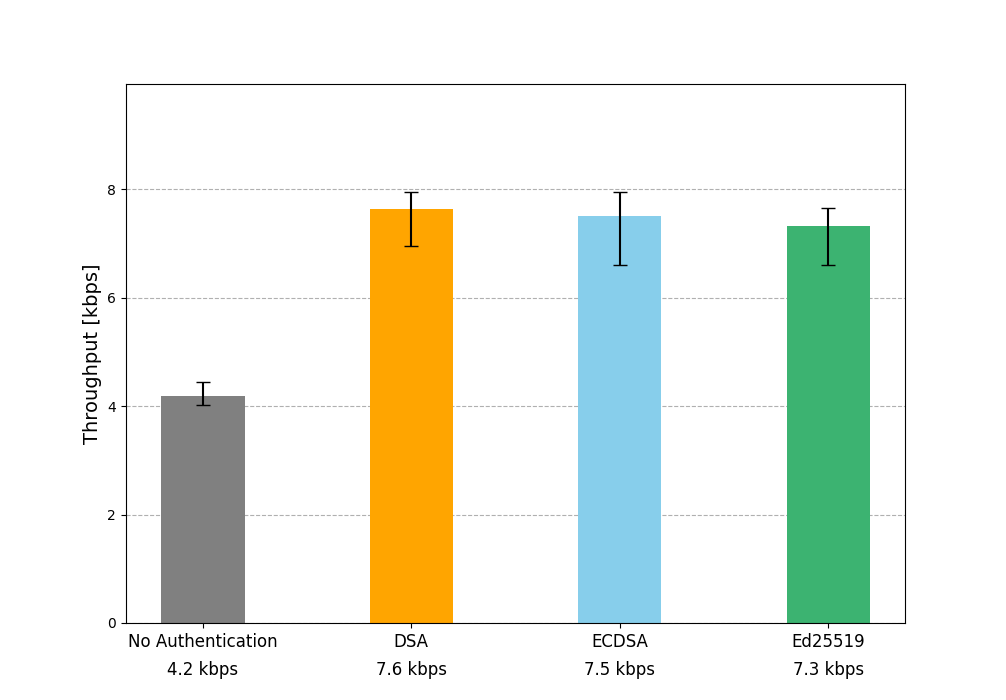
\includegraphics[width=1\textwidth]{figures/exp1_throughput.png}
  \caption{不正ノードが存在する環境でのスループット}
  \label{fig:exp1_throughput}
\end{figure}


\indent 図\ref{fig:exp1_pdr}は, 実験1におけるシミュレーションパターンごとの
パケット配送率を示している. 認証機構なしの場合に48.2 \%であるのに対し, DSAでは88.15 \%, 
ECDSAでは86.62 \%, EdDSAでは84.48 \%と, 認証機構を追加したことでパケット配送率が
約30 \%向上した. \\
\indent 図\ref{fig:exp1_throughput}は, 実験1におけるシミュレーションパターンごとの
スループットを示している. 認証機構なしの場合に4.18kbpsであるのに対し, 
DSAでは7.64kbps, ECDSAでは7.51kbps,EdDSAでは7.33kbpsと, 認証機構を
追加することでパケット配送率同様, スループットも向上した. \\
\indent これらの結果は, 認証機構の追加により 
不正ノードが排除されたことで, 経路選択を行う際に正当なノードのみを
選択しており,  データの窃取(転送中止)を回避できたことを示している. 
しかし, EdDSAの結果をDSAとECDSAの結果と比較するとほとんど差がないため, 
3つの署名方式が不正ノードを排除することにおいて同等の性能をもつと考えられる. 



